\documentclass[a4paper,12pt]{article} % добавить leqno в [] для нумерации слева
\usepackage[a4paper,top=1.3cm,bottom=2cm,left=1.5cm,right=1.5cm,marginparwidth=0.75cm]{geometry}
%%% Работа с русским языком
\usepackage{cmap}					% поиск в PDF
\usepackage[warn]{mathtext} 		% русские буквы в фомулах
\usepackage[T2A]{fontenc}			% кодировка
\usepackage[utf8]{inputenc}			% кодировка исходного текста
\usepackage[english,russian]{babel}	% локализация и переносы
\usepackage{physics}
\usepackage{multirow}

%%% Нормальное размещение таблиц (писать [H] в окружении таблицы)
\usepackage{float}
\restylefloat{table}

\usepackage{graphicx}

\usepackage{wrapfig}
\usepackage{tabularx}

\usepackage{hyperref}
\usepackage[rgb]{xcolor}
\hypersetup{
	colorlinks=true,urlcolor=blue
}

%%% Дополнительная работа с математикой
\usepackage{amsmath,amsfonts,amssymb,amsthm,mathtools} % AMS
\usepackage{icomma} % "Умная" запятая: $0,2$ --- число, $0, 2$ --- перечисление

%% Номера формул
%\mathtoolsset{showonlyrefs=true} % Показывать номера только у тех формул, на которые есть \eqref{} в тексте.

%% Шрифты
\usepackage{euscript}	 % Шрифт Евклид
\usepackage{mathrsfs} % Красивый матшрифт
\usepackage{pgfplots}
\pgfplotsset{compat=1.9}

%% Свои команды
\DeclareMathOperator{\sgn}{\mathop{sgn}}

%% Перенос знаков в формулах (по Львовскому)
\newcommand*{\hm}[1]{#1\nobreak\discretionary{}
	{\hbox{$\mathsurround=0pt #1$}}{}}

\date{\today}

\begin{document}

\begin{titlepage}
	\begin{center}
		{\large МОСКОВСКИЙ ФИЗИКО-ТЕХНИЧЕСКИЙ ИНСТИТУТ (НАЦИОНАЛЬНЫЙ ИССЛЕДОВАТЕЛЬСКИЙ УНИВЕРСИТЕТ)}
	\end{center}
	\begin{center}
		{\large Физтех-школа прикладной математики и информатики}
	\end{center}
	
	
	\vspace{4.5cm}
	{\huge
		\begin{center}
			{\bf Отчёт о выполнении лабораторной работы 4.1.1}\\
			Изучение центрированных оптических систем
		\end{center}
	}
	\vspace{1cm}
	\begin{center}
		{\large Соболевский Федор Александрович \\
			\vspace{0.2cm}
			Б05-111}
	\end{center}
	\vspace{8cm}
	\begin{center}
		Февраль 2023
	\end{center}
\end{titlepage}

\section{Аннотация}

В данной работе исследованы центрированные оптические системы, состоящие из линз различной толщины. Изучены различные методы определения фокусных расстояний тонких линз и систем из них, оценена точность каждого из методов. На примере плосковыпуклой сферической линзы исследованы различные виды аббераций, возникающих при работе с реальными оптическими приборами.

\section{Теоретические сведения}

\subsection{Способы определения фокусных расстояний центрированных оптических систем}

Существует несколько способов определения фокусных расстояний линз и центрированных систем из них. В зависимости от вида оптической системы (тонкая собирающая или рассеивающая линза, толстая линза, система линз) применимы различные методы определения положения их главных и фокальных плоскостей.

\subsubsection*{Определение фокусного расстояния тонкой собирающей линзы}

\textbf{Метод 1.} Формула тонкой собирающей линзы имеет вид
\begin{equation} \label{convergingLens}
  \frac{1}{a} + \frac{1}{a'} = \frac{1}{f},
\end{equation}
где $a$ и $a'$~-- расстояния до предмета и до его изображения соответственно, $f$~-- фокусное расстояние линзы. Пользуясь данной формулой, можно найти $f$, получив чёткое изображение предмета на экране и измерив расстояния от центра линзы до предмета и изображения.

\textbf{Метод 2.} Лучи, исходящие из точки на фокальной плоскости, при прохождении через линзу преломляются в параллельный пучок. Следовательно, положение заднего фокуса можно определить, перемещая предмет относительно линзы, пока лучи, проходящие через неё, не станут параллельными. Для проверки параллельности лучей можно воспользоваться зрительной трубой, настроенной на бесконечность (т.\,е. на максимально возможное расстояние от наблюдателя).

\subsubsection*{Определение фокусного расстояния тонкой рассеивающей линзы}

\begin{figure}[h]
    \centering
    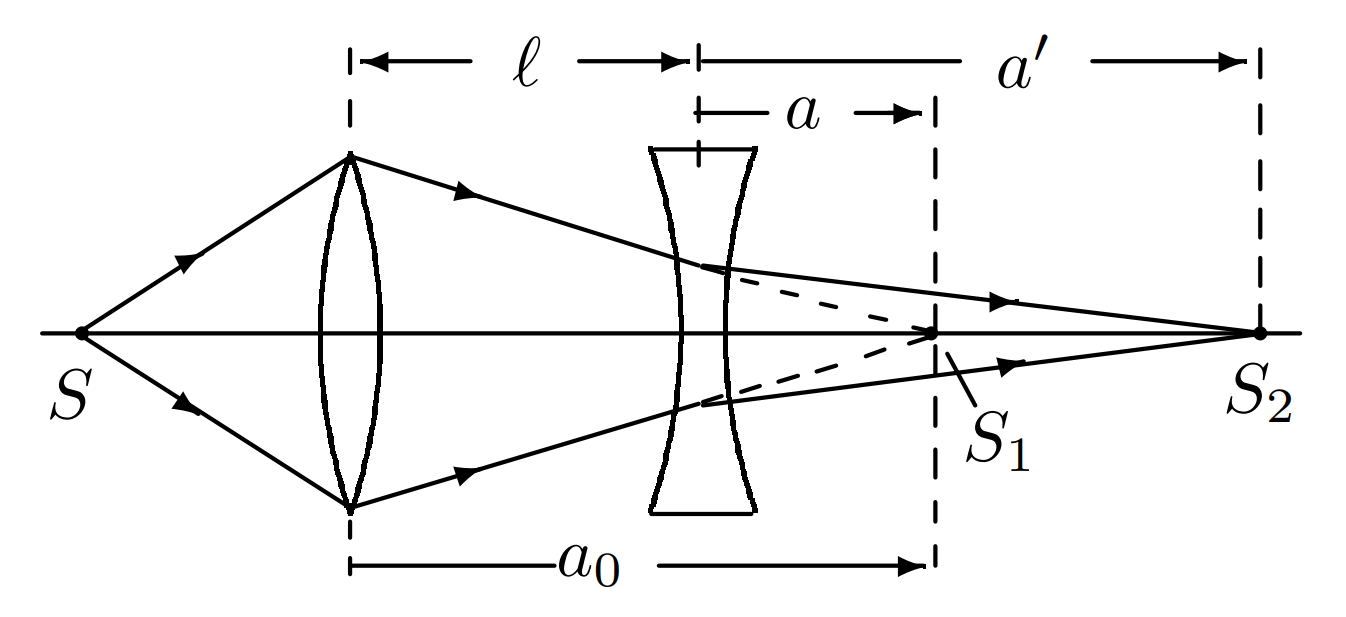
\includegraphics[width=0.7\textwidth]{divLens.png}
    \caption{Измерение фокусного расстояния рассеивающей линзы}
    \label{fig:divLens}
\end{figure}

При действительном источнике изображение в отрицательной линзе получается мнимым, поэтому для определения фокусного расстояния следует использовать дополнительную положительную линзу. 

\textbf{Метод 1.} На рис.\,\ref{fig:divLens} схематично описан метод измерения фокусного расстояния рассеивающей линзы при помощи вспомогательной собирающей. Сначала на экране следует получить изображение $S_1$ предмета в собирающей линзе, затем добавить в систему исследуемую рассеивающую линзу и переместить экран для получения нового изображения $S_2$ в полученной оптической системе. Изображение $S_1$ предмета, полученное при помощи собирающей линзы, можно рассматривать как мнимый источник света. Тогда, зная расстояния $a$ и $a'$, можно вычислить фокусное расстояние $f$ по формуле тонкой отрицательной линзы:
\begin{equation} \label{divergingLens}
  -\frac{1}{a} + \frac{1}{a'} = \frac{1}{f}.
\end{equation}

\textbf{Метод 2.} Заметим, что если мнимый источник $S_1$ находится в переднем фокусе рассеивающей линзы, то лучи, преломляющиеся в системе, на выходе преобразуются в параллельный пучок. Следовательно, по аналогии с методом 2 для собирающей линзы, можно перемещать отрицательную линзу относительно $S_1$ и наблюдать параллельные лучи при помощи зрительной трубы. 

\subsubsection*{Определение фокусного расстояния тонкой собирающей линзы и сложных оптических систем по методу Аббе}

\begin{figure}[h]
    \centering
    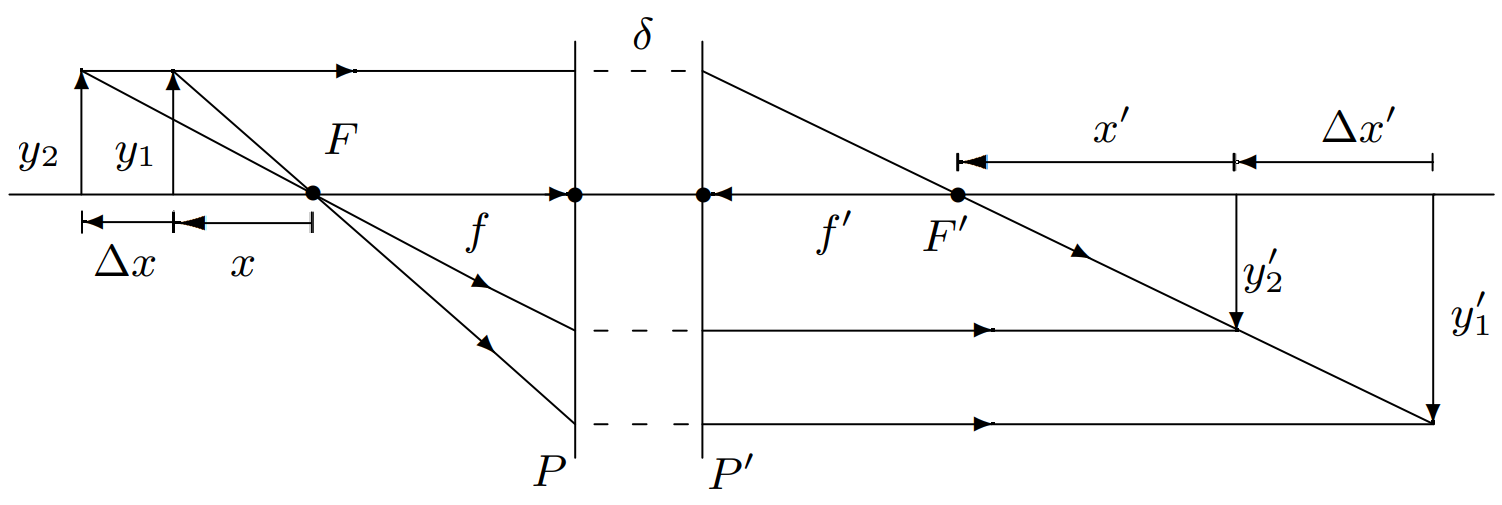
\includegraphics[width=0.95\textwidth]{AbbeMethod.png}
    \caption{Измерение фокусного расстояния оптической системы методом Аббе}
    \label{fig:AbbeMethod}
\end{figure}

Измерение фокусного расстояния по методу Аббе основано на определении поперечного увеличения для нескольких различных положений предмета, находящегося на оптической оси исследуемой оптической системы. На рис.\,\ref{fig:AbbeMethod} представлена схема измерений при помощи данного метода. Стрелкой размера $y_1=y_2=y$ изображен предмет, стрелками размера $y_1'$ и $y_2'$~-- его изображения при разных его положениях. Из геометрических соображений можно получить соотношения
\begin{equation}
    \frac{x}{y_1}=\frac{f}{y_1'},\quad\frac{x+\Delta x}{y_2}=\frac{f}{y_2'},\quad
    \frac{x'}{y_2'}=\frac{f'}{y_2},\quad\frac{x'+\Delta x}{y_1'}=\frac{f'}{y_1},
\end{equation}
откуда
\begin{equation}\label{AbbeMethod}
    f = \frac{\Delta x}{\Delta(y/y')} = -\frac{\Delta x'}{\Delta(y'/y)},
\end{equation}
где $\Delta(y/y') = y_2/y_2' - y_1/y_1'$~-- приращение поперечного увеличения, а $\Delta(y/y')$~-- приращение величины, обратной ему. Альтернативно, можно вычислить фокусное расстояние системы из двух линз, зная их фокусные расстояния. По формуле системы двух линз
\begin{equation}\label{systemFailureForTheMassesAntimatterForTheMasterplan}
    -\frac{1}{f} = \frac{1}{f_1} + \frac{1}{f_2} - \frac{|l_{12}|}{f_1f_2}.
\end{equation}

\subsubsection*{Определение положения главных и фокальных плоскостей сложной
оптической системы}

Для определения главных плоскостей оптической системы необходимо знать её фокусные расстояния и положения главных фокусов. Найти вышеперечисленные параметры системы можно, пользуясь методами, описанными в предыдущих пунктах. Отложив от главных фокусов расстояния, равные фокусным, можно найти положения главных плоскостей оптической системы.

\subsection{Абберации в реальных оптических системах}

В реальных оптических системах, в отличие от идеальных, имеют место зависимости хода лучей от угла испускания и длины волны. Вследствие этого возникают абберации~-- небольшие отклонения фокусов разных лучей друг от друга. Основные погрешности возникают из-за сферической  и хроматической аббераций линз, входящих в оптическую систему.

\subsubsection{Сферическая абберация}

\begin{figure}[h]
    \centering
    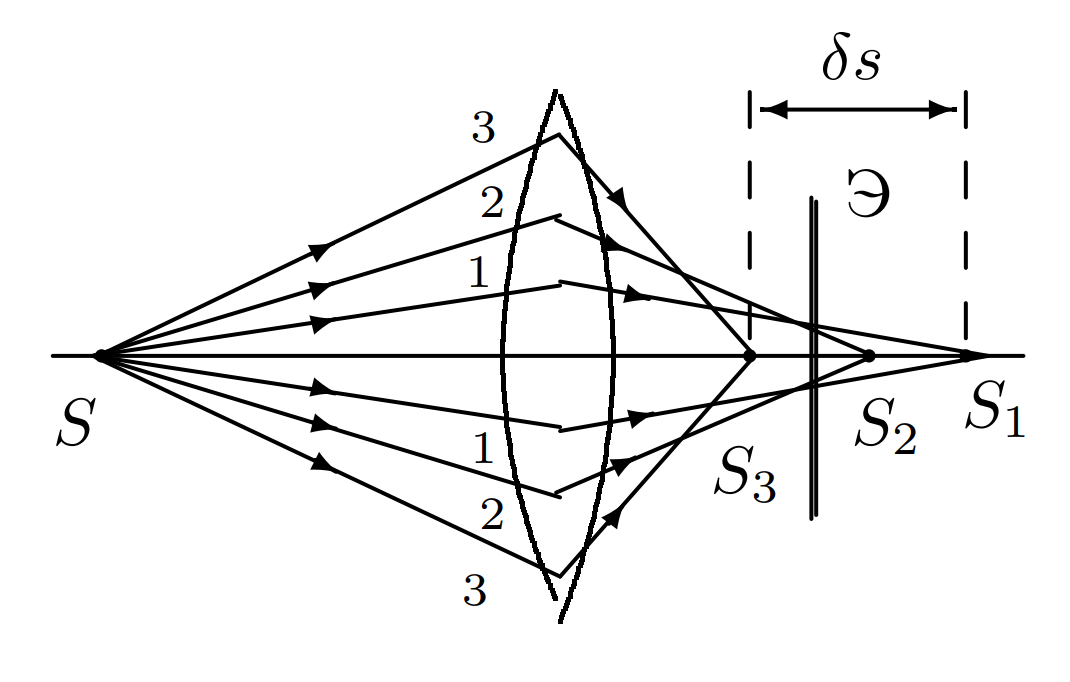
\includegraphics[width=0.6\textwidth]{spherAbberation.png}
    \caption{Сферическая абберация в толстой собирающей линзе}
    \label{fig:spherAbberation}
\end{figure}

Сферическая абберация возникает при прохождении широких пучков света через сферические поверхности линз. Данное явление проилюстрировано на рис.\,\ref{fig:spherAbberation}. Сферическую абберацию характеризуют продольной абберацией $\delta s$~-- расстоянием между точками пересечения крайних и центральных лучей с главной оптической осью.

\begin{figure}[h]
    \centering
    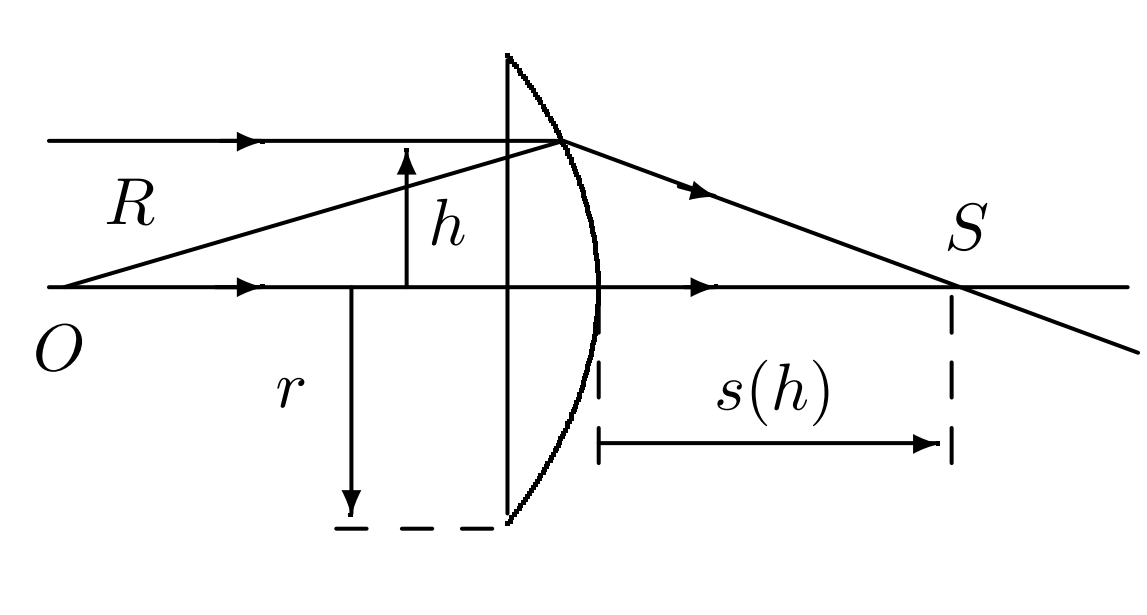
\includegraphics[width=0.6\textwidth]{planoConvexLens.png}
    \caption{Сферическая абберация плосковыпуклой линзы}
    \label{fig:planoConvex}
\end{figure}

Приближённая формула для плосковыпуклой линзы представлена ниже без доказательства в силу громоздкости расчёта продольной абберации. Для параллельных лучей, проходящих на расстоянии $h$ от оси линзы, расстояние $s$ выражается как
\begin{equation}
    s(h) = \frac{R}{n-1}\left(1 - \frac{n^2h^2}{2R^2}\right).
\end{equation}

где $R$~-- радиус сферической поверхности линзы, а $n$~-- показатель преломления стекла. В случае тонкой линзы второе слагаемое пренебрежимо мало, а потому абберации можно не учитывать. Характеристическая кривая сферической абберации~-- зависимость
\begin{equation}\label{charCurve}
    \delta s(h) = s(h)-s(0) = -\frac{1}{2}\frac{n^2h^2}{(n-1)R} = -\frac{1}{2}\left(\frac{n}{n-1}\right)^2\left(\frac{h}{f}\right)^2f.
\end{equation}
При $r=h$, где $r$~-- радиус линзы, формула \eqref{charCurve} определяет продольную сферическую абберацию линзы.

\subsubsection*{Хроматическая абберация}

\begin{figure}[h]
    \centering
    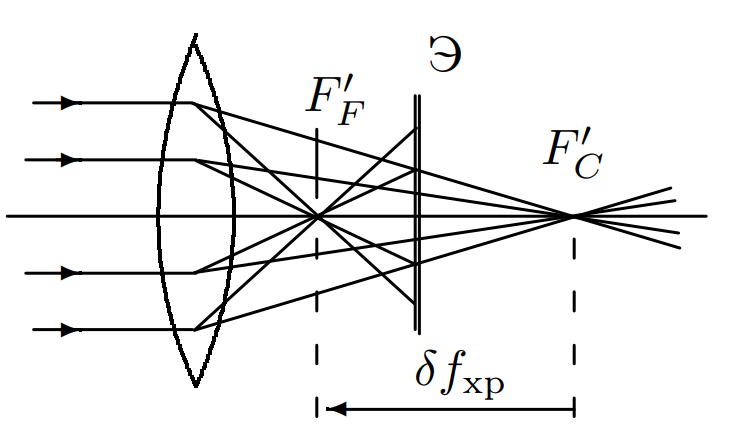
\includegraphics[width=0.6\textwidth]{chromAbberation.png}
    \caption{Хроматическая абберация}
    \label{fig:chromAbberation}
\end{figure}

Хроматическая абберация возникает из-за зависимости коэффициента преломления от длины волны света. Схематически это явление изображено на рис.\,\ref{fig:chromAbberation}. Хроматическую аберрацию принято характеризовать разностью фокусных расстояний для двух характерных спектральных линий водорода, расположенных в крайних частях видимой области спектра: $\lambda_F = 486,1$ нм (голубая линия $F$ водорода), $\lambda_C = 656,3$ нм (красная линия $C$ водорода):
\begin{equation}\label{chromAbb1}
    \delta f = f_F - f_C.
\end{equation}
Для характеристики дисперсионных свойств стёкол пользуются коэффициентом дисперсии, или числом Аббе:
\begin{equation}\label{chromAbb2}
    \nu = \frac{n_D - 1}{n_F - n_C},
\end{equation}
где $n_F$ и $n_C$~-- показатели преломления для линий $F$ и $C$ водорода, а $n_D$~-- показатель преломления для жёлтой линии $D$ натрия $\lambda_D = 589,3$ нм. Используя приближённую формулу плосковыпуклой линзы, \eqref{chromAbb1} и \eqref{chromAbb2}, получим
\begin{equation}
    \delta f = -\frac{(n_D - 1)(n_D - 1)}{(n_F - 1)(n_C - 1)}\frac{f_D}{\nu}\approx -\frac{f_D}{\nu}.
\end{equation}
Согласно табличным данным, используемое здесь приближение даёт ошибку не более 2\%, так как $n_F - n_C \sim 10^{-2}$.

\subsection{Экспериментальная установка}

Оптическая скамья с осветителем, транспарант, набор линз, экран и зрительная труба позволяют определить параметры оптических систем всеми описанными способами. Все оптические элементы устанавливались на скамье при помощи рейтеров. Перед проведением опытов все используемые оптические приборы центрировались.

\section{Оборудование и инструментальные погрешности}

\textbf{В работе использовались:} оптическая скамья с набором рейтеров, положительные и отрицательные линзы, экран, осветитель с ирисовой диафрагмой, зрительная труба, светофильтры, кольцевые диафрагмы, линейка. Линзы 1 и 2~-- тонкие собирающие, линза 3~-- плосковыпуклая, линза 4~-- тонкая рассеивающая.

\textbf{Инструментальные погрешности:}
\begin{itemize}
    \item \textbf{Линейка:} $\Delta_l = 1,0$ мм;
    \item \textbf{Измерительная шкала скамьи:} $\Delta_l = 1,0$ мм.
\end{itemize}

\section{Результаты измерений и обработка экспериментальных данных}

\subsection{Измерение фокусных расстояний тонких линз}

Для определения фокусного расстояния линзы 1 применён метод Аббе. Измеренные величины: 
$$y = 20,0\text{ мм},\quad y_1'=23,0\text{ мм},\quad y_2'=18,0\text{ мм},\quad
\Delta x = 19,0\text{ мм},\quad\Delta x'=20,0\text{ мм}.$$
Отсюда по формуле \eqref{AbbeMethod}
$$f_1^1 = \frac{\Delta x}{y(1/y_2' - 1/y_1')} = 78 \pm 8 \text{ мм},\quad f_1^2 = -\frac{y\Delta x'}{y_2' - y_1'} = 80 \pm 8 \text{ мм}.$$
Полученные значения совпадают в пределах инструментальной погрешности, что говорит о справедливости равенства в формуле \eqref{AbbeMethod}.

Для определения фокусного расстояния линзы 4 использована собирающая линза и формула тонкой отрицательной линзы. Измеренные величины:
$$a_0 = 292,0\text{ мм},\quad a' = 165,0\text{ мм},\quad l = 223,0\text{ мм},\quad a = a_0 - l = 69,0\text{ мм}.$$
Отсюда по формуле \eqref{divergingLens}
$$f = \frac{aa'}{a-a'} = -118\pm4\text{ мм}.$$
Далее фокусные расстояния линз 1, 2 и 4 определены с помощью зрительной трубы.
Полученные результаты (индекс inv обозначает измерения, выполненные при развороте линзы):
\begin{itemize}
    \item $f_1 = 95,0 \pm 1,0$ мм,   $f_1^\text{inv} = 103,0 \pm 1,0$ мм;
    \item $f_2 = 130,0 \pm 1,0$ мм,   $f_2^\text{inv} = 125,0 \pm 1,0$ мм;
    \item $a_0 = 313,0$ мм,   $l = 216,0$ мм,   $l^\text{inv} = 215,0$ мм, \\ $f_4 = a_0 - l = 97,0 \pm 1,4$ мм,   $f_4^\text{inv} = a_0 - l^\text{inv} = 98,0 \pm 1,4$ мм.
\end{itemize}

\subsection{Измерение параметров сложной оптической системы}

Для составленной из линз 1 и 2 системы измерены следующие параметры (здесь $l_{12}$~-- расстояние между центрами линз):
$$l_{12} = 63,0\text{ мм},\quad y=20,0\text{ мм},\quad y_1'=20\text{ мм},\quad y_2'=16,0\text{ мм},\quad \Delta x = 20,0\text{ мм},\quad \Delta x' = 13,0\text{ мм}.$$
Отсюда вычислены значения фокусного расстояния по формулам \eqref{AbbeMethod} и \eqref{systemFailureForTheMassesAntimatterForTheMasterplan}:
$$f_1^1 = \frac{\Delta x}{y(1/y_2' - 1/y_1')} = 80 \pm 8 \text{ мм},\quad f_1^2 = -\frac{y\Delta x'}{y_2' - y_1'} = 65 \pm 8 \text{ мм};$$
$$f = -\left(\frac{1}{f_1} + \frac{1}{f_2} - \frac{|l_{12}|}{f_1f_2}\right)^{-1} = 76\pm 12\text{ мм}.$$
Далее с помощью зрительной трубы определено положение переднего главного фокуса системы (с обеих сторон):
$$x_1 = 45,0\text{ мм},\quad x_2 = 42,0\text{ мм}.$$

\subsection{Измерение продольной сферической абберации}

Качественные и количественные измерения аббераций произведены с плосковыпуклой линзой №3. Расстояние между резкими изображениями при значениях радиусов диафрагм $h_1 = 0,5$ мм и $h_2 = 2,0$ мм равно $\Delta a = 1,7$ мм. При помощи интерполяции зависимости $\delta s(h^2)$ (см. рис.\,\ref{graph:interpoll}) в точках $h = 0$ и $h = r = 25$ мм получено значение продольной сферической абберации для линзы 3:
$$\delta s = 3,5 \pm 0,2\text{ мм}.$$

\begin{figure}[h] \label{graph:interpoll}
\begin{center}
\begin{tikzpicture}
    \begin{axis}[
    xlabel={$h^2$, мм$^2$},
    ylabel={$\delta s$, мм},
    xmajorgrids=true,
    ymajorgrids=true,
    grid style=dashed,
    xmin = 0,
    ymin = 0,
    xmax = 650,
    ymax = 4
    ]
    \addplot[color=blue, mark=o] coordinates{
    (0, 0)
    (100, 0.6)
    (400, 2.3)
    (625, 3.5)};
    \end{axis}
\end{tikzpicture}
\caption{Зависимость величины продольной абберации от ширины диафрагмы}
\end{center}
\end{figure}

Пользуясь найденным значением $\delta s$, а также известным значением $f$, можно найти показатель преломления стекла, из которого сделана линза 3:
$$n = 1,5 \pm 0,1.$$
Исходя из этого можно предположить, что линза сделана из стекла Крон ($n = 1,50--1,54$) или обычного оконного стекла ($n\approx1,52$).

\subsection{Измерение хроматической абберации}

С помощью красного и синего стёкол измерены фокусные расстояния линзы для длин волн $\lambda_C$ и $\lambda_F$: $f_F = 68$ мм, $f_C = 71$ мм; фокусное расстояние линзы для жёлтых лучей известно: $f_D = 70$ мм. Отсюда получены величина хроматической абберации и число Аббе:
$$\delta f = f_F - f_C = -3\pm1\text{ мм},\quad \nu \approx -\frac{f_D}{\delta f} = 23\pm12\text{ мм}.$$
Такая большая ошибка измерений не позволяет даже приблизительно определить марку стекла.

\section{Обсуждение результатов и выводы}

В данной работе были применены различные методы определения фокусных расстояний тонких линз. Инструментальные погрешности во всех опытах лежат в пределах $\sim10\%$, однако результаты, полученные разными методами, заметно отличаются. Учитывая, что при работе с оптическими приборами крайне важна точность, такие измерения непригодны для точного определения параметров тонких линз.

В ходе данной работы было сложно численно оценить случайные погрешности, которые возникали при измерениях. Наиболее вероятным источником погрешностей является зрение человека при определении чёткости изображений "на глаз". В силу неидеальности зрения человека и самой оптической системы экспериментатору удаётся определить лишь приблизительный диапазон на главной оптической оси, в котором лежит чёткое изображение предмета. При случайном выборе значения фокусного расстояния из данного диапазона возникает заметная погрешность измерений, устранить которую может лишь замена наблюдателя на оптический прибор, способный точно определять положение фокусировки лучей.

Есть и другие источники случайных погрешностей при измерениях: неидеальная настройка зрительной трубы, ненадёжность линейки при измерении расстояний "на глаз", возможные отклонения линз от первоначальных центрированных положений. Всё это говорит о несовершенности применённых методов определения фокусных расстояний тонких линз и оптических систем. При наблюдении аббераций в плосковыпуклой линзе возникли дополнительные трудности в измерениях: нетончость определения сфокусированности удалённых от центра лучей при исследовании сферической абберации, трудности при поиске фокусов лучей разного цвета при исследовании хроматической абберации, размытие изображений из-за пыли и/или влаги на поверхности толстой линзы и т.\,п. Всё это привело к невозможности точного количественного описания исследованных приборов и явлений.

\textbf{Выводы:} В ходе данной работы были установлены несовершенства методов количественного изучения центрированных оптических систем из линз. Предоставленные в лаборатории приборы пригодны лишь для качественного исследования рассмотренных систем и приблизительных количественных оценок. Наибольшую точность показал метод поиска фокусов путём наблюдения параллельных лучей при помощи зрительной трубы. При исследовании аббераций в толстой линзе также не удалось получить достаточно точные количественные результаты, однако качественные наблюдения показали, что абберации являются существенными при работе с толстыми линзами и системами, их содержащими. 

Основные погрешности измерений связаны с человеческим фактором: зрительные наблюдения не обеспечивают достаточной точности при исследовании точных оптических систем. Также источниками погрешностей являются недостаточно точные измерительные приборы, не приспособленные, к тому же, к точным измерениям размеров и расстояний в изученных оптических системах. Для повышения точности следовало бы минимизировать погрешности, связанные с неточностью человеческого наблюдения~-- например, автоматизировать процесс поиска сфокусированных изображений при помощи электронных оптических приборов. Также для повышения точности следовало бы точно измерить все геометрические параметры установки и применять более точные инструменты для измерения длин.

\end{document}